%
%  $Description: Author guidelines and sample document in LaTeX 2.09$ 
%
%  $Author: John Burchell & William Granli $
%  $Date: 2015/01/21 15:20:59 $
%  $Revision: 1.0
%

\documentclass[10pt,twocolumn]{article} 
\usepackage{latex8}
\usepackage{url}
\usepackage{verbatim}
\usepackage{fixltx2e}
\usepackage{graphicx}
\usepackage{enumitem}
\usepackage{amsmath}
\usepackage{mathtools}
%\documentstyle[times,art10,twocolumn,latex8]{article}

%------------------------------------------------------------------------- 
% take the % away on next line to produce the final camera-ready version 
\pagestyle{empty}

%------------------------------------------------------------------------- 
\begin{document}



\title{Assignment 4}

% author names and affiliations
\author{John Burchell and William Granli \\
john.a.burchell, william.granli@gmail.com}


\maketitle
\thispagestyle{empty}

%------------------------------------------------------------------------- 

\section{Introduction}
Software inspections have since its inception \cite{fagan2002design} more than
25 years ago spawned quite some interest both from the
research community and industrial practice. The research
includes changes to the inspection process, e.g. \cite{bisant1989two}, support to
the process, e.g. \cite{basili1996empirical} and empirical studies, e.g. \cite{basili1999building}. The
suggested improvements include active design reviews \cite{parnas1985active} and
perspective-based reading \cite{shull2000perspective}. Industry has studied the
benefits of conducting software inspections \cite{weller1993lessons}.

\section{Purpose of the Study}
This section will describe the purpose of the study, the research questions and the hypotheses. 

\subsection{Purpose Statement}
The objective of this study is to compare and hence
evaluate how well the use-case based reading performs in
comparison to other methods. The study presents a controlled
experiment where use-case based reading is compared to
checklist-based reading.

\subsubsection{Variables}
Three types of variables are defined for the experiment,
independent, controlled, and dependent variables.

\begin{enumerate}[label=(\alph*)]

	\item Independent Variable: The independent variable is
	the reading technique used. The experiment groups used either
	Use-Cased Based Reading or Checklist-Based Reading.
	\item Controlled Variable: The controlled variable is the
	experience of the reviewers and it is measured on an ordinal
	scale. The reviewers were asked to fill in a questionnaire
	comprising seven questions.
	\item Dependent Variables: The dependent variables
	measured are faults. The four variables are: (1) Number of
	faults found by each reviewer, (2) Number of faults found by
	each experiment group, (3) efficiency (faults/hour) and is
	measured as: 60*(number of fault found/inspection time which
	is 45 min), and (4) effectiveness (detection rate) and is measured
	as: number of faults found/total number of faults.

\end{enumerate}

\subsection{Research Questions}
\begin{itemize}
\item RQ1 - Is there a difference in effectiveness between Use-Case Based Reading and Checklist-Based Reading?
\item RQ2 - Is there a difference in efficiency between Use-Case Based Reading and Checklist-Based Reading?
\item RQ3 - Are different faults found by inspectors using Use-Case Based Reading than faults found by inspectors using Checklist-Based Reading? 
\end{itemize}

\subsection{Hypothesis}
The general hypothesis of the experiment is that Use-Case
Based Reading is more efficient and effective in finding faults
of the most critical fault classes, i.e. Checklist-Based Reading
is assumed to find more faults per time unit, and to find a
larger rate of the critical faults.
The dependent variables are analysed to evaluate the
hypotheses of the experiment. The main null and alternative
hypotheses \cite{montgomery2008design} are stated below. These are evaluated for all
faults, class A faults and class A\&B faults. The hypotheses
concern efficiency, effectiveness and fault detecting
differences:

\begin{itemize}
\item H\textsubscript{0 Eff} - There is no difference in efficiency (i.e.found faults per hour) between the reviewers applying use cases and the reviewers using a checklist.
\item H\textsubscript{1 Eff} - There is a difference in efficiency between the reviewers applying prioritised use cases and the reviewers using a checklist.
\item H\textsubscript{0 Rate} - There is no difference in effectiveness (i.e. rate of faults found) between the reviewers applying use cases and the reviewers using a checklist.
\item H\textsubscript{1 Rate} - There is a difference in effectiveness between the reviewers applying use cases and the reviewers using a checklist.
\item H\textsubscript{0 Fault} - The reviewers applying use cases do not detect different faults than the reviewers using a checklist.
\item H\textsubscript{1 Fault} - The reviewers applying use cases detect different faults than the reviewers using a checklist.

\end{itemize}

\Section{Methodology}
This section will describe which statistical tests were used, and why. The level of significance used for all tests is 0.05. The results have been analysed using a descriptive approach together with a statistical approach.

\SubSection{Tests Used for H\textsubscript{Eff} and H\textsubscript{Rate}}
Initially, Kolmogorov-Smirnov (KS) Goodness-of-Fit and Shapiro-Wilks (SW) tests were used to determine if the assumption of normality could be held for the data set. The data used for the tests was the number faults found by each participant. The reason this data was chosen was that it directly correlates to the data used in H\textsubscript{Eff} and H\textsubscript{Rate}. No data points were removed from the data set before performing any tests for H\textsubscript{Eff} or H\textsubscript{Rate}. The reasoning for this was that the hypotheses only concern number of occurrences and not the qualitative attributes of the data. This means that data points which, for example, contained ``incorrect'' \textit{Item numbers} were still used in the calculation.

The KS and SW tests both reported p-values \textless 0.05. See Table 1 for the p-values of the KS and SW tests. The critical value analysis for the KS and SW showed similar results and thus the null hypotheses of the data being normally distributed was rejected. See Table 2 for more information about the critical value results of the KS and SW tests.


\begin{table}
	\centering
	\begin{tabular}[ht]{| l | l | l |}
	\hline
	Test & Sample & p-value  \\
	\hline
	KS & UC & \textless 2.2e-16 \\
	\hline
	SW & UC & 0.000969 \\
	\hline
	KS & CL & \textless 2.2e-16 \\
	\hline
	SW & CL & 0.309 \\	
	\hline
	\end{tabular}
	\caption{KS \& SW tests - p-value}
\end{table}


\begin{table}
	\centering
	\begin{tabular}[ht]{| l | l | l | l |}
	\hline
	Test & Sample & Critical Value & D (result)  \\
	\hline
	KS & UC & 0.270 & 0.9388 \\
	\hline
	SW & UC & 0.964 &  0.8412 \\
	\hline
	KS & CL & 0.270 & 0.9388 \\
	\hline
	SW & CL & 0.964 & 0.9553 \\	
	\hline
	\end{tabular}
	\caption{KS \& SW tests - Critical Value}
\end{table}


A graphical representation of the level of normalisation can be seen in Figure 1 and 2. The results from the tests are supported by the sparseness of the data points. 

\begin{figure}[ht]
\centering
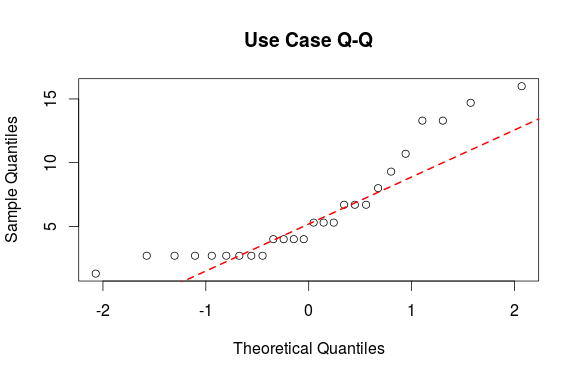
\includegraphics[width=90mm]{uc_qq.png}
\caption{Use Case Q-Q plot}
\end{figure}

\begin{figure}[ht]
\centering
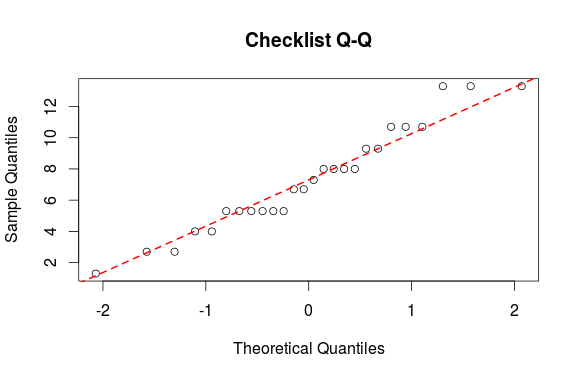
\includegraphics[width=90mm]{cl_qq.png}
\caption{Checklist Q-Q plot}
\end{figure}


The next step was to perform an outlier test. The method used was boxplots. As seen in Figure 3 and 4, no outliers were detected and thus no data points were removed in the tests performed. 

\begin{figure}[ht]
\centering
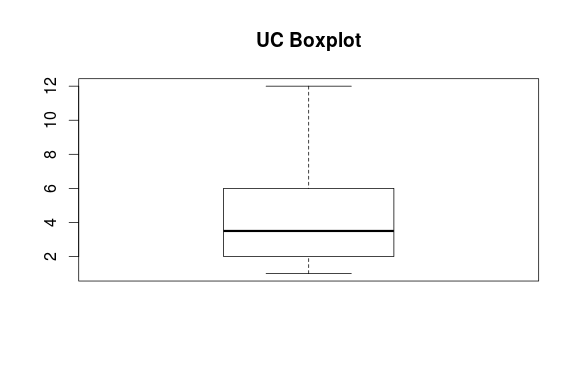
\includegraphics[width=90mm]{uc_box.png}
\caption{Use Case Boxplot}
\end{figure}

\begin{figure}[ht]
\centering
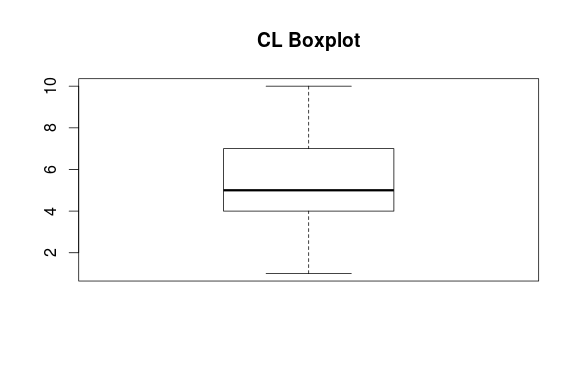
\includegraphics[width=90mm]{cl_box.png}
\caption{Checklist Boxplot}
\end{figure}


\SubSection{Test Used for H\textsubscript{Fault}}

To determine if the inspection processes find different risks, we looked at the total frequency of the types of risks found. We decided to use the risk type of the fault as opposed to using the class of fault (Missing, Wrong) as the fault type had more categories to chose from (A,B,C). We chose not to use the section in which the data was located and the item number as the data were mostly incomplete or incorrect.

The frequency of A, B and C risks found were tabulated against the inspection groups which found them. Any response that was not not applicable (NA) was discarded from the table. An example of this is found in table 3. In order to determine if they do find the same risks, a Chi-Square (CS) test of independence was performed on the tabulated results. The reason the CS was used was primarily because the data we wished to use were categorical and the frequency of each category was at least 5. Other tests, such as Fishers Exact Test were not applicable, for example, our table was greater than 2x2 rows and Fishers test should only be used for tables that are 2x2 in size.

\begin{table}
	\centering
	\begin{tabular}[ht]{| l | l | l | l | l |}
	\hline
	 & A Faults & B Faults & C Faults & Excluded\\
	\hline
	UC & 36 & 40 & 35 & 9\\
	\hline
	CL & 31 & 47 & 28 & 27\\
	\hline
	\end{tabular}
	\caption{Fault frequency of risk type per group}
\end{table}

\Section{Results}
This section will cover the results of the experiment. The results for H\textsubscript{Eff} and H\textsubscript{Rate} are described in the same sub-sections, since the results are similar and since the results both are relative to the number of average faults found. 

\subsection{Results for H\textsubscript{Eff} and H\textsubscript{Rate}}
Since the data is non-normalised, the Wilcoxon-Mann-Whitney (WMW) two-sample rank-sum test was chosen instead of the Student's T-test as the final test. The data used for the WMW test was the efficiency of each participant. The result of the WMW test was W=250, p=0.1063 and with the significance level of 536, thus the null hypothesis H\textsubscript{0 Eff} is rejected. 

The same test was chosen for H\textsubscript{Rate}, based on the same reasoning. The result of the WMW test for H\textsubscript{Rate} was W=250, p=0.1063 and with the significance level of 536 thus the null hypothesis H\textsubscript{0 Rate} is rejected. 

As evident from the tests, and as can be seen in Table 4, the results for H\textsubscript{Eff} and H\textsubscript{Rate} are similar. Both show that there is a difference between the two inspection methods, and both show greater results for CL. Table 3 shows that UC finds more faults of risk type A and C, but the fact that the CL data contained 18 more faults that contained an incorrect fault risk entry could be a possible explanation for that. 


\subsection{Results for H\textsubscript{Fault}}
As mentioned previously, the CS test was used to determine if the reviewers discovered the same frequency of results. The result of the X\textsuperscript{2} was 1.5998, generating a p-value of 0.4494. For v=2 and alpha = 0.05, the upper critical value is 5.991 and the lower critical value is 0.103. Since 1.5998 is \textless 5.991 and \textgreater 0.103, the alternative hypothesis of the CS test is rejected. Since \textsubscript{0 Fault} and \textsubscript{1 Fault} are inverted compared to the hypothesis of the CS test, the null hypothesis of H\textsubscript{Fault} is rejected.

When looking at the results of the study, UC appears to find many more class A and class B faults than CL, however, CL finds more class B faults. However, on average, the CL reviews found more faults overall and as such could be considered more effective than UC. This, coupled with the rejection of the H\textsubscript{Fault} null hypothesis, provides ample evidence that the review techniques do differ in which faults they are finding. A suggestion for a follow up study would be to determine exactly  and why one inspection process finds them over the other.

\begin{table}
	\centering
	\begin{tabular}[ht]{|l|l|l|}
	\hline
	& UC & CL \\
	\hline
	Mean(Total faults found) & 4.61 & 5.48 \\
	\hline
	Median(Total faults found) & 3.5 & 5.0 \\
	\hline
	Detection Rate & 0.12 & 0.14 \\
	\hline
	\end{tabular}
	\caption{Results Summary}
\end{table}





The slight variation in favour of the CL technique is further evidence that CL is more efficient and therefore more effective than UC.




\bibliographystyle{latex8}
\bibliography{latex8}


\Section{Acknowledgements}
U w0T m8


\end{document}

